% aliveKat, presentation to CGA, wk11
\documentclass[12pt]{beamer}
\mode<presentation> {
\usetheme{Madrid}
\setbeamertemplate{navigation symbols}{}
}

\usepackage[utf8]{inputenc}
\usepackage{amsmath, amssymb, amsthm}
\usepackage{amsfonts}
\usepackage{graphicx}
\usepackage{float}  % bunch of formatting stuff
\usepackage[center]{caption}
\usepackage{hyperref}
\usepackage{mathtools}

\usepackage{subfig}
\usepackage{comment}
% \usepackage{siunitx}

% \usepackage{booktabs} % toprule, \midrule and \bottomrule in tables
% \newcommand\hmmax{0}  % stop the 'too many math scripts' error
% \newcommand\bmmax{0}

\newcommand{\code}[1]{\texttt{#1}}


%TITLE PAGE
\title[Optical modelling of GW detectors]{Optical modelling of advanced gravitational wave detector configurations}

\author[James W. Gardner et al.]{James~W.~Gardner, Vaishali~B.~Adya, David~McClelland, Daniel~Töyrä}
\date{\today}

\begin{document}

\begin{frame}
\titlepage
\end{frame}

%%%%%%%%%%%%%%%%%%%%%%%%%%%%%%%%%%%%%%%%%%

\begin{frame}{Motivation: HF sensitivity}
% GW detectors and neutron stars as example of HF source
\begin{figure}
\includegraphics<1>[height=\textwidth,angle=-90]{figures/gwo_ifos-pictures.pdf}
\caption*{LIGO-Hanford, LIGO-Livingston, VIRGO, KAGRA}
\end{figure}
% quantum noise at HF
\end{frame}

\begin{frame}{Motivation: quantum noise limited detection}
\centering
\includegraphics<1>[width=0.8\textwidth]{figures/sqz_aLIGO_analytics_quantum_noise_budget-labelled.pdf}
\end{frame}

\begin{frame}{Our goal}
\begin{block}{Test the new \code{nle} component in Finesse}
\begin{itemize}
\item why bother?
\item what’s the \code{nle}?
\item what’s Finesse?
\end{itemize}
% If successful, then allows us an efficient means to test configurations
\end{block}
\end{frame}

% quantum noise in phase quadrature
\begin{frame}{aLIGO with long SRC and internal squeezing}
\centering
\includegraphics<1>[height=.8\textheight]{figures/aLIGO_internal_squeezing.pdf}
% \vspace{-.5cm}
% \includegraphics<2>[height=.8\textheight]{figures/aLIGO_transfer_fns_and_sensitivity_comparison.pdf}
\end{frame}

% freq. domain optical modelling, used in GW field and for optical cavities
% Finesse can do (cool stuff) ...
\begin{frame}{Finesse}
\only<2-|handout:0>{\stepcounter{framenumber}}
\begin{itemize}
\item<1> frequency domain optical modelling 
% \item e.g.\ can handle beam geometry, noise coupling, higher order modes
\item<1> can model some realistic, cool things
\item<1> used for GW detector proposals and outside GW research
\end{itemize}
\begin{figure}
    \captionsetup[subfigure]{labelformat=empty}
    \centering 
    \subfloat[\centering]{{\includegraphics<1>[width=0.2\textwidth]{figures/finesse_horse.png}}}%    
    \qquad
    \subfloat[\centering]{{\includegraphics<1>[width=0.5\textwidth]{figures/pykat_cat_and_pie.png}}}%
\end{figure}
\only{
\vfill
\url{http://www.gwoptics.org/finesse/}
}<1>
\only{
\vspace{-4cm}
}<2>
\begin{figure}
    % \captionsetup[subfigure]{labelformat=empty}
    \centering 
    % \subfloat[\centering]{{\includegraphics<2>[width=0.4\textwidth]{figures/testing_Finesse_squeezers-sq.pdf}}}%
    % \qquad
    % \subfloat[\centering]{{\includegraphics<2>[width=0.4\textwidth]{figures/testing_Finesse_squeezers-nle.pdf}}}%    
    \includegraphics<2>[width=0.8\textwidth]{figures/testing_Finesse_squeezers_comparison.pdf}
\end{figure}

\end{frame}

% \begin{frame}{Our goal}
% \begin{block}{Test the new \code{nle} component in Finesse}
% If successful, then allows us an efficient means to test configurations
% \end{block}
% \end{frame}

%%%%%%%%%%%%%%%%%%%%%%%%%%%%%%%%%%%%%%%%%%

% show method!
\begin{frame}{Squeezed cavity}
\only<2-|handout:0>{\stepcounter{framenumber}}
\centering
\qquad
\includegraphics<1>[height=0.8\textwidth, angle=-90]{figures/squeezed_cavity.pdf}
% \begin{columns}
% \column{0.5\textwidth}
% \includegraphics<2>[width=\textwidth]{figures/not_main_PSD_vs_r.pdf}
% \column{0.5\textwidth}
% \includegraphics<2>[width=\textwidth]{figures/pykat_relative_qhd_vs_r.pdf}
% \end{columns}
\includegraphics<2>[width=0.8\textwidth]{figures/squeezed_cavity_relative_qhd_vs_r_comparison.pdf}
\end{frame}

% match powers, check tunings, then compare sensitivities
\begin{frame}{aLIGO with long SRC and internal squeezing}
\only<2-|handout:0>{\stepcounter{framenumber}}
\centering 
\begin{columns}
\column{0.5\textwidth}
\includegraphics<1>[width=\textwidth]{figures/aLIGO_internal_squeezing.pdf}
\column{0.5\textwidth}
\includegraphics<1>[width=\textwidth]{figures/aLIGO_as_coupled_cavities.pdf}
\end{columns}
\vspace{-.5cm}
\includegraphics<2>[height=.88\textheight]{figures/aLIGO_transfer_fns_and_sensitivity_comparison.pdf}
\includegraphics<3>[height=0.8\textwidth, angle=-90]{figures/sqz_aLIGO_analytics_v_simulation_with_fractional_errors.pdf}        
\end{frame}

\begin{frame}{Achieved our goal!}
\begin{alertblock}{Test the \code{nle} component in Finesse}
\begin{itemize}
\item Sensitivity agrees with analytics
\item Input to \code{nle} needs to be corrected by $1/4$ to match conventions
\item Now allows us an efficient means to test configurations
\end{itemize}
\end{alertblock}
\end{frame}

\begin{frame}{Future work}
\begin{block}{Optimisation for HF sensitivity}
\end{block}
\begin{exampleblock}{Modelling other configurations}
\begin{itemize}
\item Detuned long SRC
\item Non-degenerate squeezing
\end{itemize}
\end{exampleblock}
\end{frame}


%%%%%%%% repete primeiro slide %%%%%%%%
\begin{frame}
\titlepage 
\end{frame}

\begin{frame}{Example of optimisation}
\centering 
\includegraphics<1>[height=0.85\textheight]{figures/aLIGO_optimum_sensitivity_comparison.pdf}
\end{frame}

\begin{frame}{Squeezed cavity analytics}
\begin{columns}
\column{0.5\textwidth}
$$S_\mathrm{HomI}(\Omega) = \frac{A_0^2 \left( g_1(\Omega)^2 + g_2(\Omega)^2 \right)}{g_3(\Omega)^2}$$
\column{0.5\textwidth}
\tiny
\begin{align*}
g_1 &= -\cosh ^2(r) e^{\frac{2 i L \Omega }{c}} (\cos (\theta ) \left(2 r_1^2+t_1^2\right) \cos (2 \psi )\\
    &+t_1^2 \sin (\theta ) \sin (2 \psi )) \\
    &-\cos (\theta ) \sinh ^2(r) \left(2 r_1^2+t_1^2\right) e^{\frac{2 i L \Omega
    }{c}}\\
    &-t_1^2 \cos (\theta ) \sinh (2 r) \cos (\psi ) \cos (2 \phi ) e^{\frac{2 i L \Omega }{c}}\\
    &-t_1^2 \sin (\theta )
    \sinh (2 r) \cos (\psi ) \sin (2 \phi ) e^{\frac{2 i L \Omega }{c}}\\
    &+r_1^3 \cos (\theta ) e^{\frac{4 i L \Omega
    }{c}}+r_1 t_1^2 \cos (\theta ) e^{\frac{4 i L \Omega }{c}}+r_1 \cos (\theta ) \\
g_2 &= \cosh ^2(r) e^{\frac{2 i L \Omega }{c}} (t_1^2 \cos (\theta ) \sin (2 \psi )\\
    &-\sin (\theta ) \left(2 r_1^2+t_1^2\right) \cos (2 \psi ))\\
    &+\sin (\theta ) \left(-\sinh ^2(r) (2 r_1^2+t_1^2\right)
    e^{\frac{2 i L \Omega }{c}}\\
    &+t_1^2 \sinh (2 r) \cos (\psi ) \cos (2 \phi ) e^{\frac{2 i L \Omega }{c}}\\
    &+r_1^3 e^{\frac{4 i L \Omega }{c}}+r_1 t_1^2 e^{\frac{4 i L \Omega }{c}}+r_1)\\
    &-4 t_1^2 \cos (\theta ) \sinh (r) \cosh (r) \cos (\psi ) \sin (\phi ) \cos (\phi ) e^{\frac{2 i L \Omega }{c}} \\
g_3 &= 1 + r_1^2 e^{\frac{4 i L \Omega}{c}} - 2 e^{\frac{2 i L \Omega}{c}} \sinh(r)^2 \\
    &- 2 e^{\frac{2 i L \Omega}{c}} r_1 \cos(2 \psi) \cosh(r)^2 
\end{align*}
\normalsize
\end{columns}
\end{frame}

\begin{frame}{Squeezed cavity frequency response}
% \only<2-|handout:0>{\stepcounter{framenumber}}
\centering
% \includegraphics<1>[width=0.9\textwidth]{figures/not_main_PSD_vs_freq.pdf}%
% % \vspace{-.1cm}
% \includegraphics<2>[width=0.8\textwidth]{figures/pykat_relative_qhd_vs_freq.pdf}%
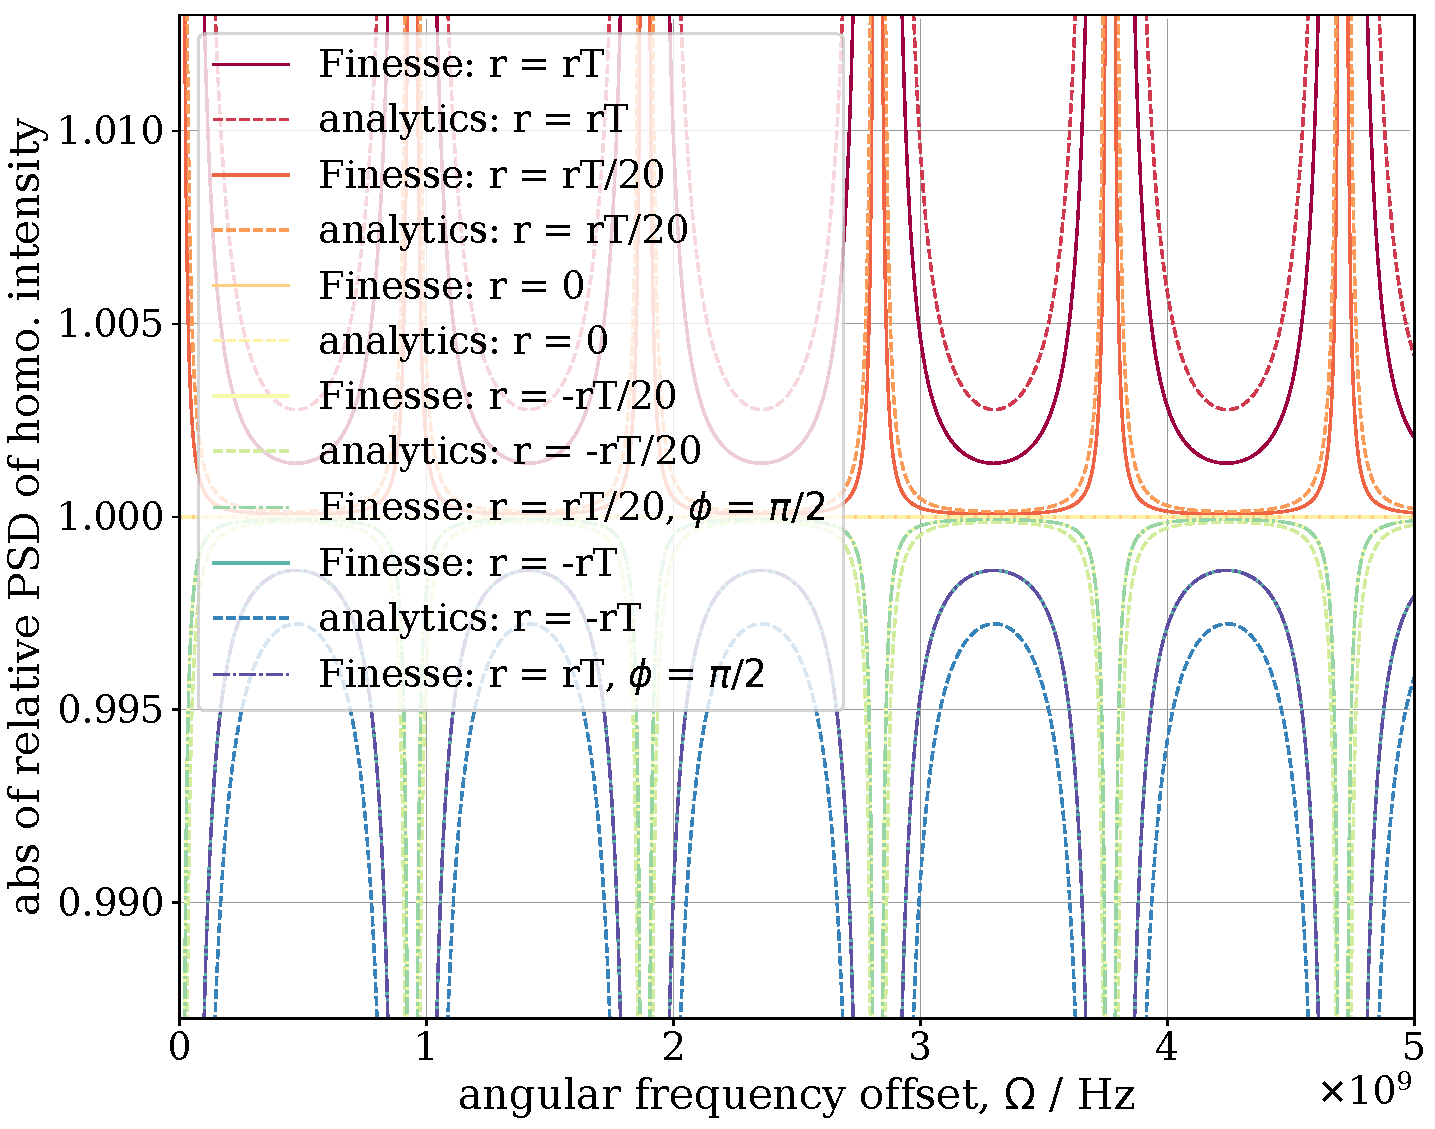
\includegraphics[width=0.8\textwidth]{figures/squeezed_cavity_relative_qhd_vs_freq_comparison.pdf}
\end{frame}

\begin{frame}{Finesse code example}
\centering 
\includegraphics<1>[height=0.85\textheight]{figures/finesse_code_example.png}
\end{frame}

\end{document}
